\clearpage\begingroup\SourceLeaf{112}\HistoricalHead{107}{R}{GAUSS AN OLBERS.}\HistoricalFoot{}{14\textsuperscript{*}}
\begin{center}[22.]\end{center}
\begin{center}\textsc{Gauss} an \textsc{Olbers}.\quad Göttingen, 18. März 1836.\end{center}
\begin{center}\begin{minipage}{.88\linewidth}\centering\hrule\vspace{3pt}
\small [\textsc{Wilhelm Olbers}, Sein Leben und seine Werke II, 2, S. 635.]
\par\vspace{3pt}\hrule\end{minipage}\end{center}
\noindent .\ .\ .\ .\ .\ .\ .\ .\ .\ .\ .\ .\ .\ .\ .\ .\ .\ .\ .\ .\ .\par
\indent Herzlichen Dank für die Unterstützung, die Sie der Reise meines Sohnes
durch Empfehlungsschreiben verschafft haben. — Mit einiger Ängstlichkeit
horche ich dem Sturm, der hier diese ganze Woche ununterbrochen getobt hat.

Die weite Verbreitung solcher Stürme gewahr zu werden, geben unsre
magnetischen Beobachtungen zuweilen Gelegenheit. Während des letzten Termins,
30/31. Januar, stürmte es hier sehr stark: aus \textls[120]{allen} Orten, von wo
correspondirende Beobachtungen eingelaufen sind (Haag, Leipzig, Marburg,
München, Mailand, Catanea) erschallen zugleich die Klagen über den heftigen
störenden Sturm.

Demungeachtet ist dieser Termin der merkwürdigste von allen bisher
abgewarteten gewesen. Mehrere grosse und schnelle Bewegungen sind vorgekommen;
allein nicht bloss bei diesen, sondern auch bei den kleinern findet
sich für alle Oerter die frappanteste Harmonie, nur auch hier wieder, je weiter
nach Süden, desto kleiner die Bewegungen, und zwar die Abnahme der Grösse
der Bewegungen in einem \textls[120]{viel} stärkern Verhältnisse, als die horizontale
Intensität grösser wird (vgl. A. N. No. 276, S. 186 ganz unten\textsuperscript{[*)]}).
\begingroup\renewcommand{\thefootnote}{}\footnotetext{[*) \textit{Beobachtungen der Variationen der Magnetnadel in Copenhagen und Mailand, am 5. u. 6. Nov. 1834}, mitgetheilt von Herrn Hofrath und Ritter \textsc{Gauss}, mit einer Kupfertafel, Astronomische Nachrichten 12, 1835, Spalte 185, Werke V, S. 537, siehe insbesondere S. 538 letzter Absatz.]}\endgroup\ 
Wir haben also, wie es scheint, die Sitze der Magnetischen Gewitter fast immer vorzugsweise
im hohen Norden zu suchen. Aber um die Sitze in einzelnen Fällen
auszumitteln, muss unsere Association erst \textls[120]{viel weiter} verbreitet sein, als
sie bis jetzt ist, und auch dann wird die Arbeit keineswegs eine leichte sein,
aus einem Grunde, den ich Ihnen, wie ich hoffe, leicht werde klar machen
können. Schon jetzt weisen viele Erfahrungen darauf hin, dass in einem Tage
eine fast unzählbare Menge solcher magnetischen Gewitter oder Eruptionen
Statt finden, die an \textls[120]{sehr verschiedenen Orten} sein mögen. Nehmen Sie
z. B. an, es sei bloss Eine Eruption bei Island, die in Göttingen etwa eine
\clearpage\SourceLeaf{113}\HistoricalHead{108}{L}{PHYSIK. BRIEFWECHSEL.}\HistoricalFoot{}{}
\noindent solche Figur für die Bewegung der Magnetnadel geben würde, und in Sicilien
\par\noindent\begin{minipage}[t]{.19\linewidth}\vspace{0pt}\centering
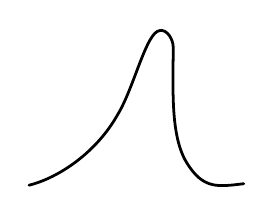
\begin{tikzpicture}[x=.0075in,y=.0075in,line cap=round,line join=round]
\draw[line width=1pt] (0,0) .. controls (20,5) and (45,22) .. (59,47)
.. controls (70,65) and (78,102) .. (87,103)
.. controls (92,104) and (96,97) .. (96,92)
.. controls (96,64) and (94,33) .. (105,15)
.. controls (116,-3) and (126,-1) .. (143,1);
\end{tikzpicture}
\end{minipage}\hfill\begin{minipage}[t]{.78\linewidth}\vspace{0pt}
eine ganz ähnliche nur viel kleinere. Es sei eine halbe Stunde
nachher eine ähnliche über (oder unter\textsuperscript{*)}) Arabien. Diese für
sich allein wird auch eine ähnliche Figur hervorbringen, aber
für Sicilien die grössere, für Göttingen die kleinere. Nach Maass-
\end{minipage}\par\noindent
gabe des Verhältnisses der Stärke der beiden Eruptionen können sich nun
daraus die Formen der zusammengesetzten Erscheinungen sehr ungleich werden
und, wie bei einigem Nachdenken klar ist, die Zeiten der Maxima und Minima
an verschiedenen Orten auch sehr ungleich ausfallen. Schon oft sind Fälle
vorgekommen, wo man ganz von selbst einen solchen Hergang anzunehmen
veranlasst wird. Sehen Sie z. B. in den A[stronomischen] N[achrichten] Stück
276 in der Zeichnung die Stunde von 15\textsuperscript{h}—16\textsuperscript{h}\textsuperscript{[**)]}.
\begingroup\renewcommand{\thefootnote}{}\footnotetext{*) Denn \textls[120]{darüber} wissen wir jetzt noch gar nichts, und wo aller Boden fehlt, hasse ich alles Hypothesiren.}
\footnotetext{[**) Die dem Aufsatze in den Astronomischen Nachrichten beigegebene Kupfertafel ist im V. Bande der Werke nicht wieder abgedruckt. Die von \textsc{Gauss} bezeichnete Stunde ist wohl die von 3\textsuperscript{h}—4\textsuperscript{h} vormittags des 6. November 1834.]}\endgroup\ 
Aber offenbar wird es \textls[120]{sehr vieler, sehr weit auseinanderliegender und sehr zuverlässiger und
scharfer} Beobachtungen bedürfen, um solche gemengten Wirkungen in ihre
einzelnen Bestandtheile aufzulösen, und aus diesen Gründen ist allerdings eine
recht grosse Verbreitung der Apparate und der Kenntniss, sie zu behandeln,
sehr wünschenswerth; vor allem aber auch eine gehörige gründliche Einsicht
in das, was damit geleistet werden kann, verglichen mit den ehemals gebrauchten
Apparaten, wobei, meine ich, gar nicht von \textls[120]{solchen} Problemen
hätte die Rede sein können.

Uebrigens breitet sich der Verein schon immer mehr aus. \textsc{Meierstein}
hat Apparate nach Halle, Freiberg, Wien und Bonn geliefert (wo sie freilich
noch nicht in Thätigkeit sind), nach Haag und München, wo trefflich beobachtet
wird, nach Upsala, wo nächstens angefangen werden soll. In Arbeit
hat er Apparate für Greenwich und Dublin. Nach Breslau sind von hier
Stäbe gesandt. Nach Krakau liefert \textsc{Breithaupt} in Cassel einen Apparat etc.

Bloss mit Berlin will es nicht vorwärts.

Die Beobachtungen des letzten Termins werden wohl auch noch lithographirt
werden. Es entsteht jedoch die Schwierigkeit, wie für künftige regelmässige
\clearpage\SourceLeaf{114}\HistoricalHead{109}{R}{GAUSS AN OLBERS UND SCHUMACHER.}
\noindent Lithographirung die \textls[120]{Kosten} gedeckt werden sollen. \textsc{Weber} meinte, dass
diess vielleicht durch Zusammentreten der Theilnehmer und Freunde geschehen
könnte, wo dann der Aufwand für einen einzelnen nicht so gar gross sein
und er dafür ein halbes Dutzend Abdrücke erhalten könnte. Ich zweifle aber,
dass diess ausführbar ist, denn natürlich kann H[err] Prof. W[\textsc{eber}] sich nicht
auf das Versenden und Einkassiren einlassen, das müsste durch Vermittlung
etwa eines Kunst- oder Buchhändlers geschehen, was sich aber schwerlich
hier in Göttingen einrichten lässt, zumahl da das Geschäft bei seiner Zersplitterung
doch zu unbedeutend sein würde.

Ich habe dagegen H[errn] Prof. \textsc{Weber} vorgeschlagen, in Göttingen ein
allgemeines eigenes physikalisches Journal zu begründen\textsuperscript{[*)]}, welches ausser
vielem anderen Nutzen auch zur Magazinirung der magnetischen Beobachtungen
ein bequemes Mittel darbieten würde. Ich weiss aber noch nicht, ob seine
grosse Bescheidenheit ihm erlauben wird, so etwas zu unternehmen. Ich selbst
kann freilich Nichts dabei thun, als zu Zeiten einmal einen kleinen Beitrag
geben. Denn meine ganze Art zu arbeiten hat eine ganz entgegengesetzte
Richtung; meine Arbeiten sind nicht zum \textls[120]{Raumfüllen}, und ein Paar Bogen
erfordern jahrelange Vorarbeit. Auch ist mir die grösste Quaal, zu bestimmter
Zeit eine Arbeit vollenden zu \textls[120]{müssen}.\quad .\ .\ .\ .\ .\ .\ .\ .\ .\ .\ .\ .\ .\ .\ .\ .\ .\ .\ .
\begingroup\renewcommand{\thefootnote}{}\footnotetext{[*) Diese Zeitschrift erschien vom Juni 1837 an bis zum Jahre 1843 in 6 Bänden unter der Überschrift: »Resultate aus den Beobachtungen des magnetischen Vereins im Jahre 1836, bezw. 1837, 1838, 1839, 1840, 1841. Herausgegeben von C. F. \textsc{Gauss} und W. \textsc{Weber}«, Göttingen 1837, 1838, Leipzig 1839, 1840, 1841, 1843.]}\endgroup
\clearpage\endgroup
